%++++++++++++++++++++++++++++++++++++++++
% Don't modify this section unless you know what you're doing!
\documentclass[letterpaper,12pt]{article}
\usepackage{tabularx} % extra features for tabular environment
\usepackage{amsmath}  % improve math presentation
\usepackage{graphicx} % takes care of graphic including machinery
\usepackage[margin=1in,letterpaper]{geometry} % decreases margins
\usepackage{cite} % takes care of citations
\usepackage[final]{hyperref} % adds hyper links inside the generated pdf file
\usepackage{verbatim}
\hypersetup{
	colorlinks=true,       % false: boxed links; true: colored links
	linkcolor=blue,        % color of internal links
	citecolor=blue,        % color of links to bibliography
	filecolor=magenta,     % color of file links
	urlcolor=blue         
}
%++++++++++++++++++++++++++++++++++++++++


\begin{document}

\title{Liberation Of Eden}
\author{Paul Archer-Smith}
\date{\today}
\maketitle

\begin{abstract}
This document covers the history, plot, and key characters of the Liberation Of Eden (LOE) campaign. 
\end{abstract}


\section{History}\label{History}

\begin{itemize}
\item \textbf{0 - The creation of the Avarisi empire:} 
\item \textbf{458 - The last great hero dies:} 
\item \textbf{626 - Johanna V'Talom born:} 
\item \textbf{776 - The kingdom of El is established:} 
\item \textbf{932 - The city of Eden is founded:}
\item \textbf{995 - Johanna V'Talom declared emperor of the Avarisi:} 
\item \textbf{1098 - The beginning of the Avarisi invasion:} 
\item \textbf{1100 - The conquest of El and the beginning of the occupation:}
\item \textbf{1102 - Morgan Niles appointed king of El:} 
\item \textbf{1137 - The rebellion at Harper's Ferry:} 
\item \textbf{1154 - D'arcy Lonergan promoted to Overseer of Eden:}
\item \textbf{1156 - The Red Falcons established:}
\item \textbf{1164 - The 3rd Way established:}
\item \textbf{1170 - The escape of Jordan Till:} 
\item \textbf{1170 - The ascension of James Malecious:}
\item \textbf{1172 - The adventure begins:} 
\end{itemize}


\section{Character creation}\label{CharacterCreation}

\subsection{Vocation}

The enslaved people of El have been organized into various different groups depending on their profession. The profession is chosen fairly young --- typically there is a ceremony during the early spring for each town (the date varies depending on the arrival of spring) occurring after the first round of planting is finished. The day of divination is treated as a celebration: run by the Avarisi, there is a banquet prepared for all followed by each child born 10 years ago (e.g born 1162 for 1172) approaching the conduit for the closest oracle. When a child approaches the conduit, the oracle chooses a vocation for them. The vocation is announced and the child is magically branded on both shoulders: one with the mark of bondage, the other with the mark of their trade. When building characters for this campaign, the players roll 1d20:

\subsubsection{Miner (1-8)}
The El who are selected to work the mines are stronger than typical but rather unhealthy due to the industrial air: + 1d4 to strength, -1 to constitution. 20\% chance of literacy. 1d8/5 rounded down starting cash.

\subsubsection{Farm Hand (9-14)}
The El who till the fields tend to be stronger and healthier than most: +1 to strength, dexterity, and constitution. 40\% chance of literacy. 1d6/5 rounded down starting cash.

\subsubsection{Laborer (15-16)}
The El who till the fields tend to be stronger and healthier than most: +1 to strength, dexterity, and constitution. 70\% chance of literacy. 1d12/5 rounded down starting cash.

\subsubsection{Teacher (17)}
The El who till the fields tend to be more empathetic and perceptive: +1d2 to wisdom and charisma. 70\% chance of literacy. If illiterate, automatically a child-caregiver; if literate, 40\% chance of being a teacher --- otherwise 50\% chance of being either a caregiver for children or seniors. 1d8/8 rounded down starting cash.

\subsubsection{Carer (18)}
This includes priests, medics, and animal handlers. 40\% chance of being a medic who are more intelligent and wiser than most, but often exposed to disease: +1d2 intelligence, +1d4 wisdom, and -1 constitution. 25\% chance of being a priest who are more intelligent, wiser, and more charismatic than most: +1d2 intelligence, +1d4 wisdom, and +1 charisma. 10\% chance of being an erotic worker who are more charismatic, dexterous, and wiser than most, but also looked down on: +1d2 wisdom, +1d2 dexterity, +1d4 charisma, but other slaves treat them poorly. The rest are animal handlers: +1d2 dexterity, +1d2 wisdom. 90\% chance of literacy for priests and medics, 100\% chance for sex workers, and a 70\% chance for animal handlers. 1d20/5 rounded down starting cash.

\subsubsection{House Slave (19)}
Servants of the richest households within Eden. Roll a percentile die to determine how high in the social order your house is (1 = 80th percentile, 100 = servant to the overseer, interpolate for results between these extremes). If the roll is 73 or greater, the slave lives in the owner's house during the week. If the roll is 87 or greater, they live in the wealthy Ro'Mar district. If the roll is 93 or greater, they serve an official in the government. For slaves with rolls below 65, literacy chance is 90\%, for those between 65 and 86 this is raised to 95\%, and for those 87 and above it is 100\%. Additionally, there is a 10\% chance for those below 87 and 20\% chance for those above to have some form of higher education. Roll a 1d8 for master temperament (1 = cruel, 8 = kind). +1d2 intelligence and +1d2 charisma. 1d20 starting cash.

\subsubsection{Clerical Assistant (20)}
The most highly trained slaves, these work as managers, calculators, and clerical assistants. All are literate and 20\% are more highly trained. Intelligence +1d4 (or 10, whichever is higher). On the rolling of a second 20 in a row, the slave is a conduit for the closest oracle. 1d20 starting cash.

\subsection{Luck}

There is a simple adjustment of a players stats due to luck: a 1d8 is rolled and we adjust the stats as follows

\begin{itemize}
\item \textbf{1, Terrible Luck:} -1 to all stats.
\item \textbf{2, Bad Luck:} -1 to 3 stats of the player's choice.
\item \textbf{3, Poor Luck:} -1 to 1 stat of the player's choice.
\item \textbf{4-5, Average Luck:} No changes.
\item \textbf{6, Alright Luck:} +1 to 1 stat of the player's choice.
\item \textbf{7, Good Luck:} +1 to 3 stats of the player's choice.
\item \textbf{1, Fantastic Luck:} +1 to all stats.
\end{itemize}

\subsubsection{Hit points}

The characters each start with (1d6 + CON) * 6 (minimum 10) hit points.

\subsubsection{Gifts}

Finally, characters are able to get a final chance at having a special gift:

\begin{itemize}
\item \textbf{1-6, Nothing:} The character gets no benefit.
\item \textbf{7, Cautious:} The character obtains proficiency in perception.
\item \textbf{8, Martial Arts:} The character's basic unarmed attack does 1d6 + STR damage. 
\item \textbf{9, Strong Arm:} The character's basic throwing attack does 1d6 + DEX damage.
\item \textbf{10, Spiritual Connection:} The character has opened a channel to the spirits of old and can cast spirit bomb attacks (using WIS) that do 1d6 + WIS damage.
\end{itemize}

\subsection{Other character creation items}

Speed starts off at 3 meters. No base proficiencies 

\section{Geography}\label{Geography}

El features a climate that can be best described as Mediterranean: most of the kingdom is relatively dry and temperate most of the year. Winters typically feature little, if any, snow --- although this does begin to change as one goes to the south-east. The northern parts of the country receive more rain and correspondingly more forests.  

\begin{figure}[ht] 
        % read manual to see what [ht] means and for other possible options
        \centering \includegraphics[width=1\columnwidth]{elMap01.png}
        % note that in above figure file name, "sr_setup",
        % the file extension is missing. LaTeX is smart enough to find
        % apropriate one (i.e. pdf, png, etc.)
        % You can add this extention yourself as it seen below
        % both notations are correct but above has more flexibility
        %\includegraphics[width=1.0\columnwidth]{sr_setup.pdf}
        \caption{Map of the kingdom of El. Eden is denoted by the brown dot in the upper centre of the grey region (the province of Tygerus).}
\end{figure}

Eden is located close to the centre of the province of Tygerus. The main city of Eden is built on a hill, with a fairly steep cliff on one side. The slaves live in a favela on a hill about 400 meters west from the main part of the city. A copper mine is about 2.5 km to the north-west of the city. A small river lies about 3.5 km to the East of the city and flows past the town of Mark (about 8 km to the south). The only other town of significance in the region is Arkeus, which lies about 18 km to the south-west. 

\begin{figure}[h] 
        % read manual to see what [ht] means and for other possible options
        \centering 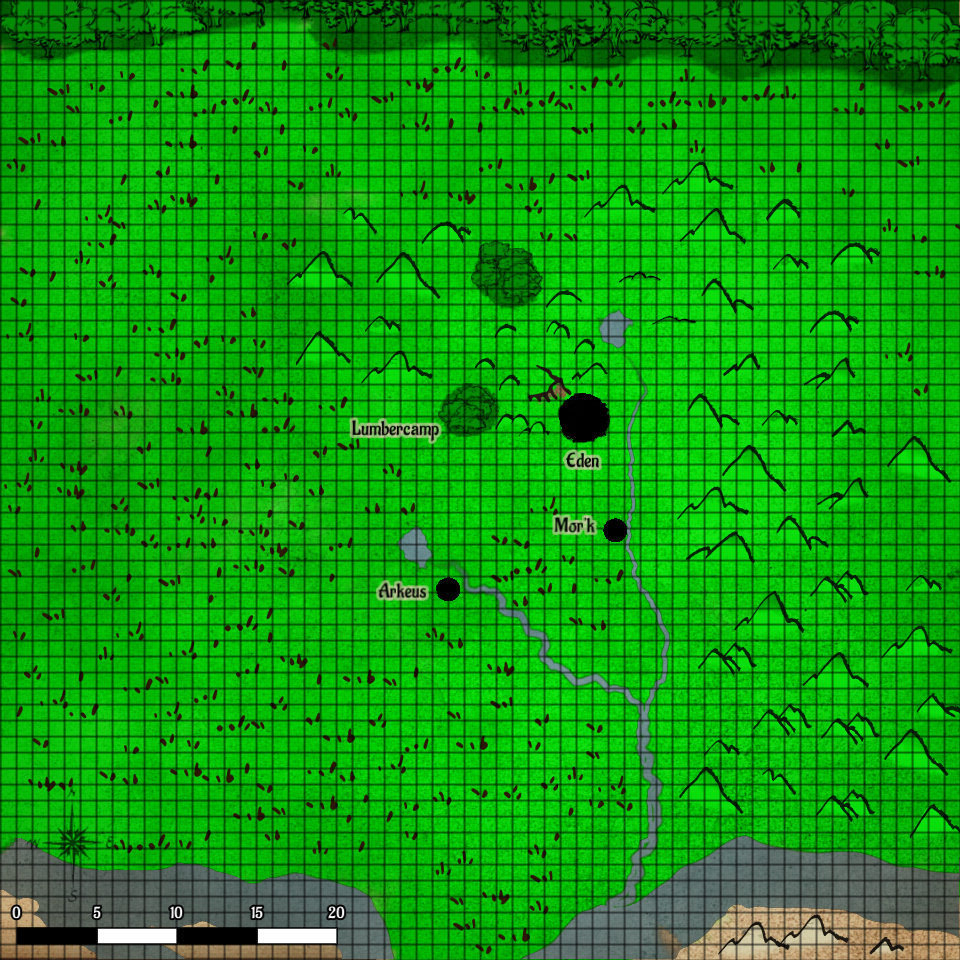
\includegraphics[scale=0.31]{edenAreaMap01.png}
        % note that in above figure file name, "sr_setup",
        % the file extension is missing. LaTeX is smart enough to find
        % apropriate one (i.e. pdf, png, etc.)
        % You can add this extention yourself as it seen below
        % both notations are correct but above has more flexibility
        %\includegraphics[width=1.0\columnwidth]{sr_setup.pdf}
        \caption{Map of the area surrounding Eden.}
\end{figure}


\section{Politics and society}\label{Politics}

\subsection{Political divisions}\label{PoliticalDivisions}


\section{Combat}\label{Combat}

The combat system of TLOE is fundamentally rooted in the 5th edition of D\&D. The overall idea of skill checks on a d20 system and attacking against some armour class remain unchanged, however the system is modified to allow for the playing of common (and even weak) characters. The most important thing adjustment is that the time of a combat round has been reduced to 3 seconds. This means that many actions that were bonus actions in D\&D are full actions here. Additionally, variance has been reduced by making most damage rolls feature the use of multiple dice: this still allows for a wide range of outcomes, but the probability distribution is heavily weighted towards its mean value. 

\subsection{Allowed actions}

Normally, each round a character can move and take an action.

\begin{itemize}
\item \textbf{Aim:} Prepare a more accurate strike on an enemy. The player gets slight advantage on their next attack (if it's on the enemy they're focusing on), but attacks versus that player are made with advantage and that player makes perception checks at serious disadvantage.
\item \textbf{Attack:} Unleash an attack on an enemy. See ``Attacks" for more details.
\item \textbf{Dash:} Take 2.5 movement actions (round the movement down to the nearest meter). See ``Running" for more details.
\item \textbf{Disengage:} Can move out of engagement range without provoking an attack of opportunity.
\item \textbf{Dodge:} Attacks against the player have slight disadvantage until their next turn.
\item \textbf{Draw or sheath a weapon:} Holds for most weapons. Some very big or very concealed weapons make require more time. 
\item \textbf{Protect:} The player protects another creature, increasing that creature's defense and lowering their own. The player may chose to give low, medium, or high levels of protection: low gives attacks against the protected creature slight disadvantage but attacks against the player advantage, medium gives attacks against the protected creature disadvantage but attacks against the player serious advantage, and high gives attacks against the protected creature serious disadvantage but attacks against the player extreme advantage. 
\item \textbf{Wait:} Up until the beginning of their next turn, the player holds their action until whenever they want to use it.
\end{itemize}


\subsection{Advantage}

Advantage here works a little differently than standard D\&D --- this is mostly because the advantage of being against a surprised opponent vs a blinded opponent aren't really comparable. As such, there are 4 levels of advantage and disadvantage, respectively: 

\begin{itemize}
\item \textbf{Slight (dis)advantage:} +1 (-1) to the check.
\item \textbf{(Dis)advantage:} +2 (-2) to the check. 
\item \textbf{Serious (dis)advantage:} Roll 2 dice, take the larger (smaller) result.
\item \textbf{Extreme (dis)advantage:} Roll 3 dice, take the largest (smallest) result.
\end{itemize}

If you end up with a case where advantages are compounding the ``advantage levels" are summed: if Sammy has an attack with slight advantage against a creature that gives disadvantage to all attack rolls, then Sammy's attack is take at slight disadvantage. No advantage (disadvantage) greater than the extreme level is possible.   

In many cases, the level of advantage is subjective. The DM should make these calls at their own discretion.

\subsection{Attacks}

 Untrained melee attacks do 1d4 damage + STR to a minimum of 1 on a hit. Untrained ranged attacks do 1d4 + DEX (a reasonably sized stone or similar projectile has a range of 7/15 meters). A branch or basic improvised weapon does 1d6 + STR, a metal rod does 1d8 + STR and a pitchfork, mining pick, or woodcutting axe does 1d10 + STR. Daggers and other standard 1d4 weapons (in D\&D) do 1d12 damage. In general, 5th edition weapon conversion is: 1d6 $\rightarrow$ 3d6, 1d8 $\rightarrow$ 3d8, 1d10 $\rightarrow$ 3d10, and 1d12 $\rightarrow$ 3d12. In general, spells do triple damage and hp is tripled. The reason for these adjustments is to make the slaves not get instantly one-banged during any early fights they might encounter while also making the transition to a more adventure D\&D style game possible. Furthermore, it balances out damage by making expected damage output be much less variance prone. 

\subsection{Running}

 There are three types of movement that are relevant to combat: combat, chase, and pursuit movement. Combat movement refers to all standard movement in combat, including the dash action, and is done using standard 3 second cycles. The chase action occurs when a short distance chase is taking place (e.g. fleeing city guards) and using 15 second cycles. Finally, pursuit movement is used for long distance chases and features 15 min time scales. Unsurprisingly, the more encumbered at player is the more difficult it is to run. Encumbrance ranges from 0 (completely free to move) to 5 (incredibly weighted down):
 
\begin{itemize}
\item \textbf{No encumbrance:} Wearing nothing but easy to move in clothes.
\item \textbf{Slight encumbrance:} Carrying a decent sized weapon (e.g. sword), a backpack, a sack, minimal armour.
\item \textbf{Encumbrance:} Wearing light armour. Wielding a large weapon, a medium shield, or a small weapon and shield. Carrying more than 10 kg in a bag, backpack, or sack. 
\item \textbf{Significant encumbrance:} Wearing medium armour. Wielding a 2-handed weapon, a large shield, or a medium shield and a weapon. Carrying more than 20 kg in a bag, backpack, or sack.
\item \textbf{Serious encumbrance:} Wearing heavy armour. Wielding a heavy 2-handed weapon. Carrying more than 30 kg or a small-sized creature.
\item \textbf{Extreme encumbrance:} Wearing ultra-heavy armour. Carrying more than 40 kg or another medium-sized creature.
\end{itemize}
 
Once a player has used the dash action 3 times in a row, they automatically enter chase movement. Similarly, if a chase goes on for over 5 minutes a player moves to pursuit movement. The speed columns indicate how many times a player moves their base speed in one movement cycle; the endurance columns indicate how many cycles a player can run before having to make CON checks to avoid exhaustion. The DC begins at 10 and increases by 2 each subsequent round. When the check is failed, the character becomes exhausted and their encumbrance level temporarily increases by 1. This process is then repeated until the chase stops or level 5 encumbrance is reached (at which point no additional encumbrance can occur). 20 - CONV time cycles (min 1) are required to recover to recover each level of exhaustion incurred.   
 
\begin{table}[ht]
\begin{center}
\caption{TLOE Movement Rules.}
\label{tbl:bins} % spaces are big no-no withing labels
\begin{tabular}{|c|c|cc|cc|} 
\hline
\multicolumn{1}{|c|}{Encumbrance} & \multicolumn{0}{|c|}{Combat (dash)} & \multicolumn{0}{|c}{Chase (sp)} & \multicolumn{0}{c|}{Chase (end)} & \multicolumn{0}{|c}{Pursuit (sp)} & \multicolumn{1}{c|}{Pursuit (end)} \\
\hline
0 &   3x &   15x &   CONV cycles &   800x &   CONV cycles \\
1 &   3x &   13x &   CONV cycles - 1 &   750x &   CONV cycles - 2\\
2 &   2.5x &   11x &   CONV cycles - 2 &   600x &   CONV cycles - 4\\
3 &   2.5x &   9x &   CONV cycles - 4 &   450x &   CONV cycles - 7\\
4 &   2x &   7x &   CONV cycles - 6 &  300x  &   CONV cycles - 10\\
5 &   --- &   5x &   --- &   150x &   --- \\
\hline
\end{tabular}
\end{center}
\end{table}



\subsection{Injuries}
 
Injuries are always possible when a character gets hit down to low health:

\begin{itemize}
\item \textbf{50\% Health --- Beaten:} Every hit that damages a player to health below 50\% (including hits that start below 50\% hp, e.g. 43\% to 28\%) has a 5\% chance of injuring the player. If the character is injured, there is a 5\% chance it is a moderate injury. 
\item \textbf{25\% Health --- Bloodied:} Every hit that damages a player to health below 25\% has a 15\% chance of injuring the player. If the character is injured, there is a 10\% chance it is a moderate injury. 
\item \textbf{10\% Health --- Bodied:} Every hit that damages a player to health below 25\% has a 35\% chance of injuring the player. If the character is injured, there is a 5\% chance of a severe injury and a 25\% chance it is a moderate injury. 
\item \textbf{0\% Health --- Incapacitated:} The character is unable to take any actions. When a character is incapacitated, there is a 60\% chance they are injured. There is a 25\% chance this injury is severe and 50\% chance the injury is moderate. Death saving throws work the same as in base 5e. If a character is incapacitated, an enemy within reach can try to coup de grace them. The character rolls a 1d20 --- anything other than a natural 20 results in death.
\item \textbf{-100\% Health --- Death:} The character is dead. 
\end{itemize}  

Minor injuries are to be given at the DM's discretion. Minor injuries should take at least 3 days and at most 2 weeks to heal fully. When the injury is fully unhealed, a minus 2 penalty applies to all checks done that utilize the relevant body part (e.g. a sprained ankle makes any sort of acrobatics check have a -2). After one-third of the recovery time has passed or proper medical assistance has been obtained, this is lowered to a -1. 

Moderate injuries take 2-6 weeks to heal fully; this includes fractures, major sprains, moderate concussions, minor stab wounds, etc. In general, this causes all relevant rolls to be done with disadvantage. In general, roll a 1d20:

\begin{itemize}
\item \textbf{1-7, Broken Bone:} A bone is broken or fractured. Roll a 1d6: on a 1 it's a moderate break, otherwise it's a fracture. Roll a 1d6 for body part: 1 - right leg, 2 - left leg, 3 - ribs, 4 - right arm, 5 - left arm, 6 - DM's choice. 3-4 weeks to heal a fracture, 6 to heal a break.
\item \textbf{8-14, Flesh Wound:} A massive chunk of skin has been lost. If not treated within a few minutes, roll a 1d10: on a 1 the wound keeps bleeding and the character starts losing 1d6 hit points every minute until the wound is successfully treated or they die, on a 2 the wound becomes infected, and on a 10 the wound heals without scaring. Every day with an infection, roll a 1d20: on a 1 this becomes a serious infection on a 17-20 it becomes uninfected. Serious infections result in disadvantage to all future rolls (including rolls to become uninfected), drain all physical stats by 2, and require the character to roll a 1d20 every day: on a 1-2 the character dies and on a 17-20 the infection returns to a regular infection. Body parts are DM's discretion. Regular wounds take 2 weeks to heal, but 2 weeks plus infection period for an infected wound. 
\item \textbf{15-16, Concussion:} All mental and physical work is affected: all checks (besides recovery checks) are made at disadvantage. Everyday the character rolls a 1d20: on a 19 or 20 they recover and on a 1 they roll a 1d2: a 2 means nothing happens but a 1 means the permanent loss of either 1 INT or the development of memory problems (if this happens three times the character develops dementia and becomes unplayable). If strenuous activity is undertaken a 20 is required to recover and the INT damage die is rolled on a 1-3. 
\item \textbf{17-18, Lose Teeth:} The character loses 1d4 teeth.
\item \textbf{19, Cornea Scratch:} The character's cornea is scratched making all perception checks occur at disadvantage and -2. Everyday the character rolls a 1d20: 17-20 mean recovery, 1 means vision is permanently damaged from that eye, reducing perception permanently by 2.
\item \textbf{20, Lost Digit:} The character loses a finger or toe. 2 weeks to heal. 
\end{itemize} 

Major injuries take a massive amount of time to heal --- or, in some cases, never do. The characters need to find some sort of mitigating strategy if this occurs. Any relevant rolls are done with extreme disadvantage: the bottom 1 of 3 or 4 rolls is typically taken.

\begin{itemize}
\item \textbf{1-7, Smashed Bone:} A bone is smashed. Roll a 1d6 for body part: 1 - right leg, 2 - left leg, 3 - abdomen, 4 - right arm, 5 - left arm, 6 - neck or face. You need medical attention to make sure this heals right. If no medical attention (and the bone is just attempted to be forced back into place) then there is only a 5\% chance the bone heals properly. With medical attention there is a 50\% chance things heal properly. 8-12 weeks recovery. The DM determines the impact of this injury.
\item \textbf{8-14, Severe Flesh Wound:} A massive chunk of skin has been lost. If not treated within a minute, roll a 1d10: on a 1-3 the wound keeps bleeding and the character starts losing 1d10 hit points every minute until the wound is successfully treated or they die, on a 4-5 the wound becomes severely infected, on a 6-7 the wound becomes infected, and every other roll leads to a regular wound. Body parts are DM's discretion. Uninfected severe wounds take 4 weeks to heal, but 4 weeks plus infection period is required for an infected wound. 
\item \textbf{15-16, Severe Concussion:} All mental and physical work is affected: all checks (besides recovery checks) are made at extra disadvantage. Everyday the character rolls a 1d20: on a 20 the concussion becomes moderate and on a 1-3 they roll a 1d2: a 2 means nothing happens but a 1 means the permanent loss of either 1 INT or the development of memory problems (if this happens three times the character develops dementia and becomes unplayable). If strenuous activity is undertaken no recovery is possible and the INT damage die is rolled on a 1-6. 
\item \textbf{17-18, Facial Damage:} The character's face is disfigured. 1d4 charisma is lost.
\item \textbf{19, Lost Eye:} The character loses an eye. All perception checks and ranged attacks are made at disadvantage.
\item \textbf{20, Lost Hand or Foot:} The character loses a hand or foot. 4 weeks to heal. 20\% chance of infection.  
\end{itemize} 

\section{Equipment and Items}\label{Equipment}

Work in progress.

\subsection{Weapons}

\subsection{Armour}

\subsection{Supplies}

\subsection{Trade goods}

\subsection{Potions}

\subsection{Magic equipment}

\section{Character advancement}\label{LevelingUp}

Work in progress.

\section{Key characters}\label{Characters}

I'm uncertain of how to adapt this section for players, as you're not supposed to know much about these characters. As such, I've stripped almost all the information from these profiles, leaving only the names. At some point, I might fill this in with the details that the party knows. Or, if you want, you can fill it in yourself as you learn bits and pieces.

\subsection{Public figures}

\begin{itemize}
\item \textbf{Emperor Johanna V'Talom:} The emperor of the kingdom of Avarisi.

\item \textbf{King Morgan Nilas:} The king of the conquered land of El.

\item \textbf{Viceroy James Malecious:} The viceroy of the province of Tygerus, the province of El where Eden is located. He is stationed in the provincial capital of Sinderin, where he has presided since 1170.

\item \textbf{Overseer D'arcy Lonergan:} The overseer of Eden since 1154, D'arcy came to power after the death of the old overseer, Bortan Jornal.
\end{itemize}

\subsection{Historical figures}

\begin{itemize}
\item \textbf{John Brown:} 
\end{itemize}

\subsection{Avarisi of Eden}

\begin{itemize}
\item Nothing for you yet!
\end{itemize}

\subsection{El of Eden}

\begin{itemize}
\item \textbf{Moyra:}

\item \textbf{Jaxxon Pine:}

\item \textbf{Jessie Thaler:}

\end{itemize}

\section{Plot}\label{Plot}

You don't get to read this section!!

\section{Enemies}\label{Enemies}

You don't get to read this section!!
   
%Keep the following chunk as examples of how to input images and tables.
\begin{comment}
\begin{figure}[ht] 
        % read manual to see what [ht] means and for other possible options
        \centering \includegraphics[width=0.8\columnwidth]{sr_setup}
        % note that in above figure file name, "sr_setup",
        % the file extension is missing. LaTeX is smart enough to find
        % apropriate one (i.e. pdf, png, etc.)
        % You can add this extention yourself as it seen below
        % both notations are correct but above has more flexibility
        %\includegraphics[width=1.0\columnwidth]{sr_setup.pdf}
        \caption{
                \label{fig:samplesetup} % spaces are big no-no withing labels
                % things like fig: are optional in the label but it helps
                % to orient yourself when you have multiple figures,
                % equations and tables
                Every figure MUST have a caption.
        }
\end{figure}

\begin{table}[ht]
\begin{center}
\caption{Every table needs a caption.}
\label{tbl:bins} % spaces are big no-no withing labels
\begin{tabular}{|cc|} 
\hline
\multicolumn{1}{|c}{$x$ (m)} & \multicolumn{1}{c|}{$V$ (V)} \\
\hline
0.0044151 &   0.0030871 \\
0.0021633 &   0.0021343 \\
0.0003600 &   0.0018642 \\
0.0023831 &   0.0013287 \\
\hline
\end{tabular}
\end{center}
\end{table}

\end{comment}

%++++++++++++++++++++++++++++++++++++++++
% References section will be created automatically 
% with inclusion of "thebibliography" environment
% as it shown below. See text starting with line
% \begin{thebibliography}{99}
% Note: with this approach it is YOUR responsibility to put them in order
% of appearance.

\begin{thebibliography}{99}

\bibitem{Carena2013}
M. Carena, I. Low, and C. Wagner: \textit{Implications of a Modified Higgs to Diphoton Decay Width},
(JHEP, August 2012), arXiv:1206.1082v3[hep-ph].

\end{thebibliography}


\end{document}
